\chapter{Deep Learning}
\label{deep_learning}
Il Machine Learning (ML) è una branca dell’Intelligenza Artificiale (IA) che si occupa di costruire modelli che apprendono dai dati che gli vengono forniti. Il Deep Learning, a sua volta, è una branca del ML e anch’esso si occupa di costruire modelli che apprendono pattern dai dati. La peculiarità del DL sta nella tipologia di modelli utilizzati, ovvero le reti neurali, anche dette Artifical Neural Networks (ANN) o Deep Neural Network (DNN). Una ANN è un modello di calcolo ispirato alla struttura delle reti neurali del cervello, ed è costituita da un gran numero di componenti di calcolo di base (neuroni), che sono collegati tra loro in una rete di comunicazione complessa attraverso la quale è in grado di approssimare funzioni molto complesse.
L’utilizzo delle reti neurali infatti, diventa fondamentale quando il pattern che si cerca di apprendere è molto complesso e soprattutto non lineare. Proprio questa capacità di apprendere pattern complessi ha reso il DL un tool molto utilizzato e che ha portato netti miglioramenti in molti campi, tra cui il Natural Language Processing, speech recognition, campo medico, sistemi di trasporto intelligenti \cite{dlsurvey} e molti altri \cite{dlsurvey2}. La Figura \ref{fig:appl_dl} illustra diversi campi di applicazione del DL.
\begin{figure}[h!]
    \centering
    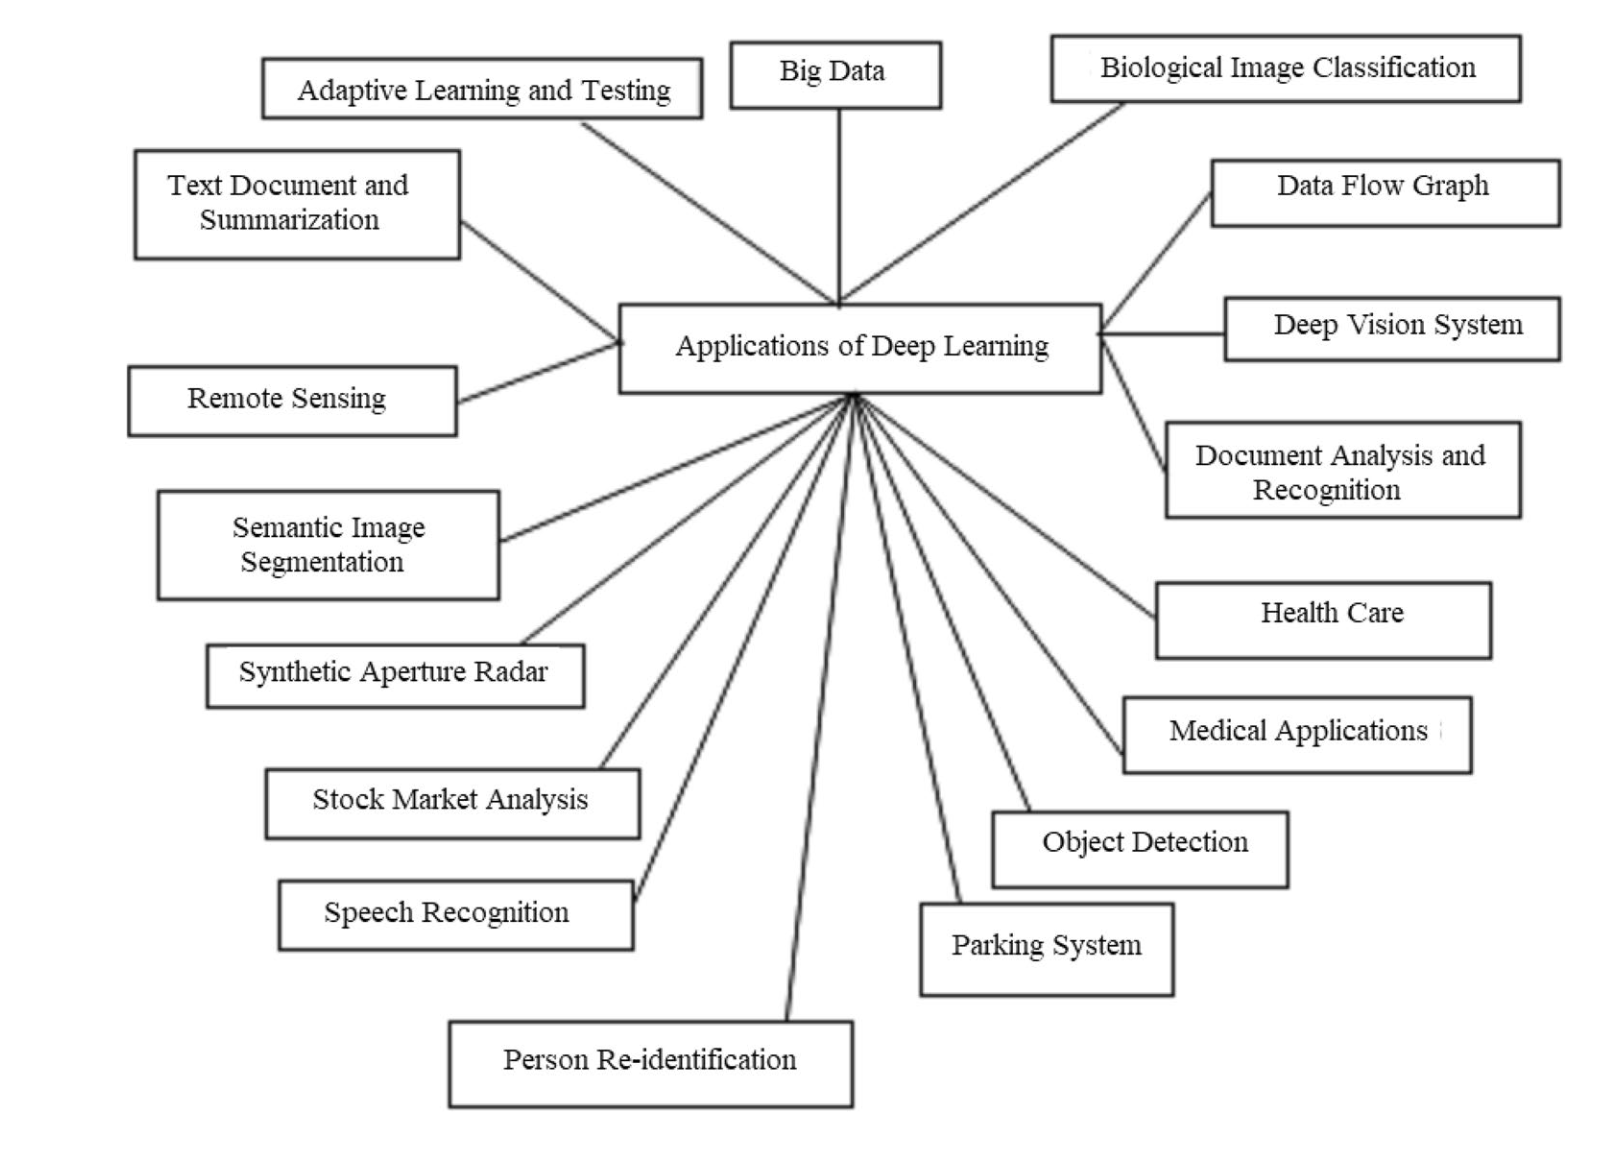
\includegraphics[scale=0.39]{img/applications_DL.png}
    \caption{Alcuni dei campi di applicazione del Deep Learning \cite{dlsurvey2}.}
    \label{fig:appl_dl}
\end{figure}
Un altro campo in cui il DL ha avuto molto successo è stato quello dell'analisi d'immagini. In particolare, per alcuni task come la classificazione e la segmentazione, le reti neurali hanno apportato netti miglioramenti. Infatti, a partire dal 2012, quando l'AlexNet \cite{alexnet} (Figura \ref{fig:alexnet}) vinse la ImageNet challenge battendo gli altri concorrenti con una un rateo di errore di circa il 16\%, contro il 26\% del vincitore dell'anno precedente, le reti neurali hanno sempre dominato le challenge riguardanti task di Computer Vision. 
Un'altra peculiarità del DL, che lo distingue dal ML e che lo rende così efficiente in campi come la Computer Vision, è che la fase di \textit{feature extraction} del ML, in cui vengono manualmente estratte le feature dal dato, è implicita nell'apprendimento della rete neurale (Figura \ref{fig:ML_vs_DL}). Questa caratteristica risulta fondamentale in quanto spesso questa fase risulta molto complessa, sia per la difficoltà dell'estrazione stessa, soprattutto per dati di tipo immagine, sia perché spesso per conoscere quali siano le feature da estrarre, è necessaria una conoscenza specifica del campo di applicazione. Nelle reti neurali invece, è proprio attraverso il meccanismo di apprendimento che la rete capisce quali sono le feature importanti e che determinano la natura del dato.

\begin{figure}[h!]
  \hspace*{0.2in}
  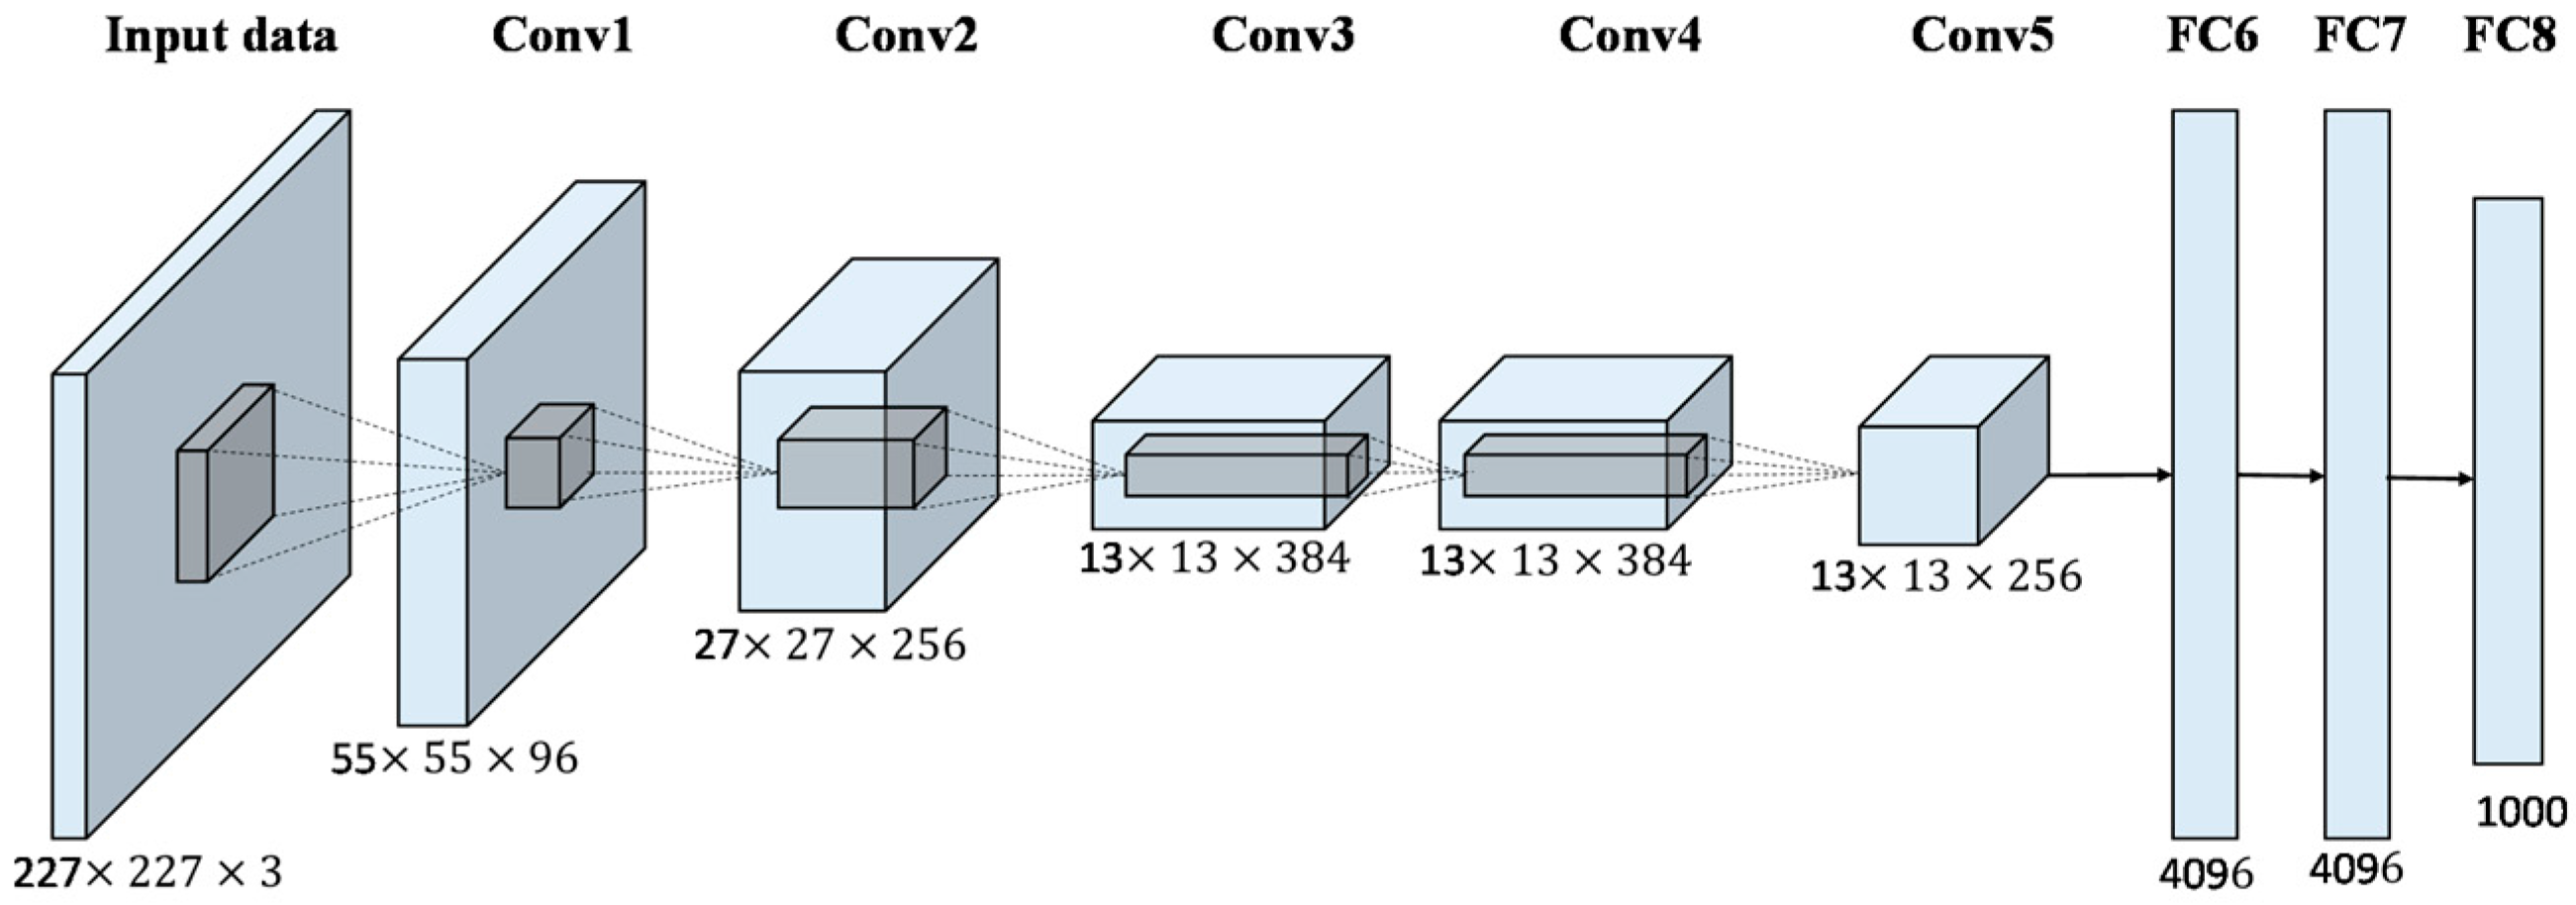
\includegraphics[scale=0.14]{img/alexnet2.png}
  \caption{Architettura della rete AlexNet.}
  \label{fig:alexnet}
\end{figure}

Oltre ai vantaggi, le reti neurali presentano anche diversi svantaggi. Uno di questi è che per alcuni aspetti le reti neurali sono dei modelli black-box. In particolare, il loro funzionamento è molto complesso e spesso, a differenza degli algoritmi di ML, il loro comportamento e i loro output diventano difficili da comprendere e di conseguenza da spiegare. Infatti negli ultimi anni, un campo dell'IA in forte crescita è l'Explainable AI \cite{expai}, che si occupa di algoritmi che forniscono trasparenza e interpretabilità a metodologie come le reti neurali.
\\ \\
\begin{figure}[h!]
    \centering
    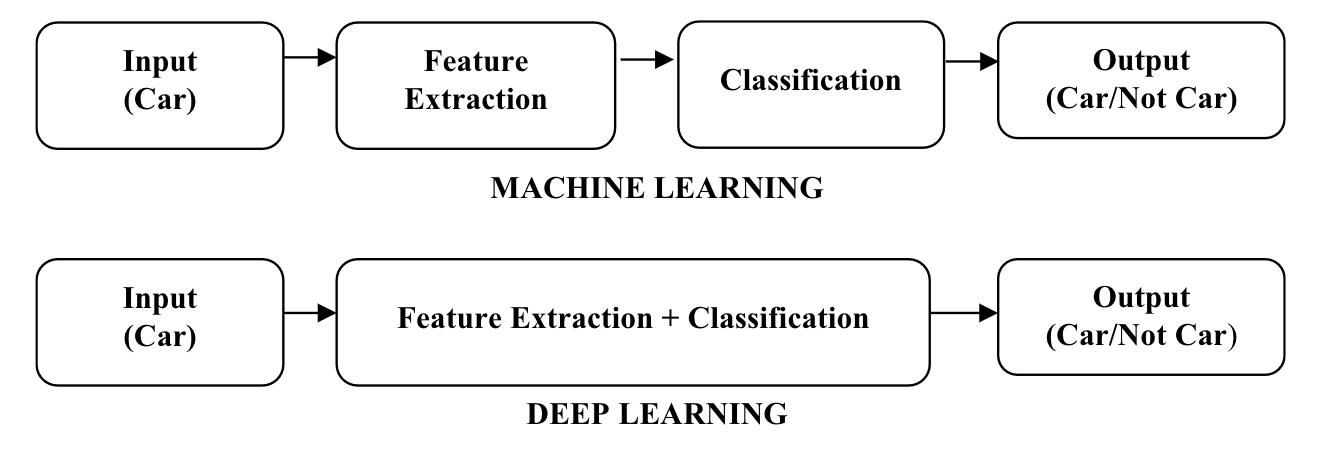
\includegraphics[scale=0.5]{img/ML_vs_DL.png}
    \caption{Differenza tra Machine Learning e Deep Learning \cite{dlsurvey2}.}
    \label{fig:ML_vs_DL}
\end{figure}




\section{Percettrone}
Il percettrone è un modello matematico ispirato al modello del neurone biologico \cite{rosenblatt1958perceptron} e costituisce il componente di calcolo di base delle reti neurali. Mentre il neurone biologico è costituito da quattro principali componenti (soma, dendriti, assone e sinapsi), il percettrone è composto da due parti (Figura \ref{fig:perceptron}): nella prima parte, viene calcolato il prodotto scalare tra il vettore d’input $X = (x_{1}, x_{2}, ..., x_{n})$ e i parametri del percettrone $W = (w_{1}, w_{2}, ..., w_{n})$ , mentre nella seconda parte il risultato del prodotto scalare viene dato in input alla funzione di attivazione $g$, che ci restituisce uno scalare. Di seguito la formula dell'output del percettrone:
\begin{equation}
    y = g( \sum_{j=1}^{n}{x_{j}w_{j}} ).
\end{equation}


La funzione di attivazione è una parte critica del percettrone, in quanto fornisce alla rete la non linearità, proprietà fondamentale per approssimare funzioni non lineari complesse. In particolare, senza funzioni di attivazione, per quanto complesse e profonde  possano essere le reti neurali, non rappresenterebbero altro che una funzione lineare dell’input e diventerebbero un semplice regressore lineare. Più avanti vedremo nei dettagli quali sono le funzioni di attivazione più utilizzate nelle moderne reti neurali.\\ \\

\begin{figure}[h!]
  \hspace*{0.3in}
  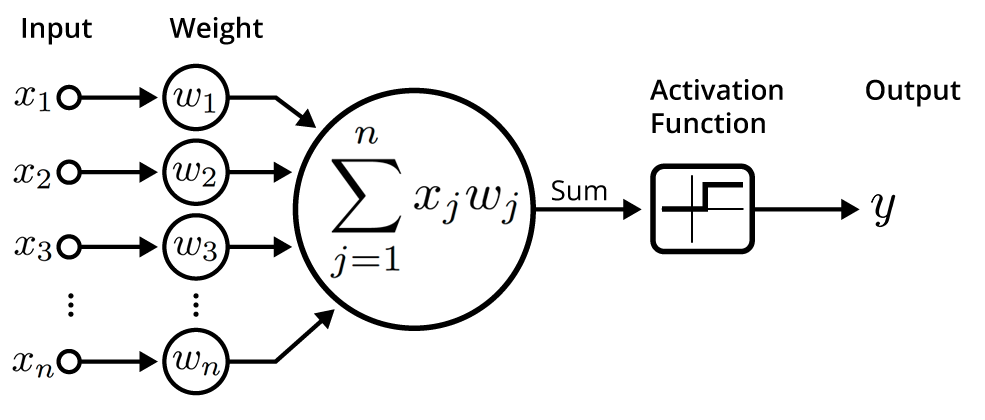
\includegraphics[scale=0.35]{img/neurone.png}
  \caption{Illustrazione della struttura di un percettrone.}
  \label{fig:perceptron}
\end{figure}














\section{Percettrone Multistrato}
Una delle tipologie più semplici di reti neurali è il Percettrone Multistrato, in inglese Multi-Layer Perceptron (MLP). L’MLP non è altro che un’insieme di percettroni collegati tra di loro e organizzati in strati (Figura \ref{fig:MLP}), dove gli output dei percettroni di uno strato sono l’input dei percettroni dello strato successivo. Gli strati, minimo tre, sono suddivisi in strato d’input, strato d’output e strati nascosti. Lo strato d’input è quello che riceve per primo il dato da elaborare, lo strato di output è quello che invece restituisce  l‘output finale della rete e  gli strati nascosti sono tutti gli altri che si trovano nel mezzo.\\

\begin{figure}[h!]
  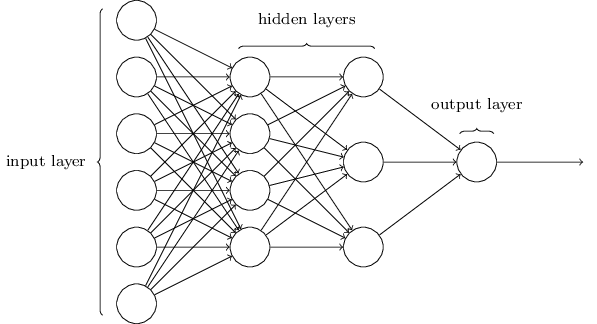
\includegraphics[scale=0.6]{img/MLP.png}
  \caption{Generica architettura di un Percettrone Multistrato.}
  \label{fig:MLP}
\end{figure}

Come detto precedentemente, grazie all’utilizzo delle funzioni di attivazione, l’output finale della rete risulta una funzione complessa e fortemente non lineare dell’input, complessità e non linearità che aumentano con l’aumentare delle dimensioni della rete. Questa proprietà risulta fondamentale e peculiare delle reti neurali, che si distinguono dagli altri modelli di ML proprio per la capacità di rappresentare funzioni molto complesse. Infatti, le reti neurali hanno preso il sopravvento soprattutto in quei task dove le funzioni o i pattern da apprendere sono molto complessi,  come nel campo dell’analisi di immagini.












\section{Funzioni di attivazione}
Come detto precedentemente, le funzioni di attivazione rappresentano un concetto cardine delle reti neurali. In particolare, la scelta delle funzioni di attivazione è una scelta fondamentale e può avere un grande impatto sulle performance del modello. All’interno di una rete, spesso vi sono diverse tipologie di funzioni di attivazione e nella maggior parte dei casi, se ne usano diverse tipologie per le diverse parti della rete. Tipicamente, gli strati nascosti utilizzano la stessa tipologia, mentre la scelta di quella dello strato di output dipende soprattutto dal task e dal tipo di output che bisogna fornire.
Di seguito, le funzioni di attivazione più utilizzate e presenti in letteratura.

\subsection{Funzione sigmoidea}
Una delle più note è la funzione sigmoidea (Figura \ref{fig:sigmoid}), anche detta sigmoid, una funzione matematica con la tipica curva ad S o curva sigmoid. In particolare, la sigmoid non fa altro che mappare l’input (un qualsiasi reale) su un range che va da 0 a 1: più l’input è grande e più sarà vicino a 1, mentre più sarà piccolo e più sarà vicino a 0. Di seguito la formula:
\\
\begin{equation}
\sigma(x) = \frac{1}{1+e^{-x}}.
\end{equation}
\\
La sigmoid viene spesso utilizzata nell’ultimo strato della rete neurale, soprattutto nei task di classificazione binaria, dove l’output finale della rete deve essere mappato nell’intervallo [0,1], in quanto rappresenta la probabilità che l’input appartenga a una delle due classi predeterminate.\\ \\

\begin{figure}[h!]
  \hspace*{0.9in}
  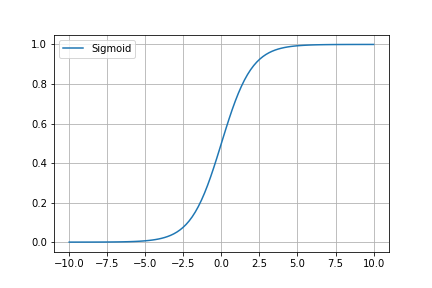
\includegraphics[scale=0.6]{img/sigmoid.png}
  \caption{Grafico della funzione sigmoidea.}
  \label{fig:sigmoid}
\end{figure}

\subsection{Tangente iperbolica}
La tangente iperbolica (Figura \ref{fig:tanh}), detta spesso “tanh”, è una funzione di attivazione molto simile alla sigmoid. La principale differenza è che mappa l’input nell’intervallo $[-1, +1]$ invece che in $[0, +1]$.\\ \\


\begin{figure}[h!]
  \hspace*{0.9in}
  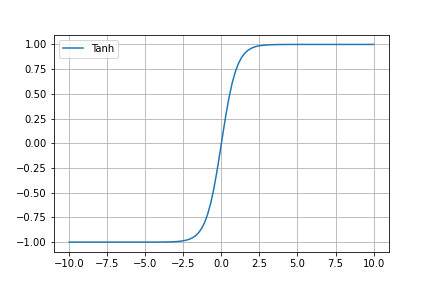
\includegraphics[scale=0.6]{img/tanh.png}
  \caption{Grafico della tangente iperbolica.}
  \label{fig:tanh}
\end{figure}










\subsection{Rectified Linear Activation Function}
La ReLU (Rectified Linear Unit) (Figura \ref{fig:relu}) è forse la funzione di attivazione più utilizzata. Il motivo sta nel fatto che risolve uno dei principali problemi delle funzioni di attivazione, ovvero la scomparsa del gradiente. Quest'ultima riguarda il fatto che nel meccanismo di retropropagazione (che affronteremo più avanti), soprattutto quando si hanno molti strati, i gradienti che vengono moltiplicati, se hanno valori piccoli, tendono ad andare verso lo 0 molto velocemente e questo porta ad avere cambiamenti, soprattutto nei primi strati della rete (gli ultimi nella retropropagazione), molto piccoli se non nulli. Di seguito la formula:
\\
\begin{equation}
  f(x) = x^{+} = max(0,x).
\end{equation}
\\
Inoltre la ReLU, vista la sua formula, risulta anche molto più semplice da calcolare rispetto alle altre e questa proprietà diventa critica soprattutto nelle reti neurali, dove spesso il costo computazionale diventa un ostacolo. Dall’altra parte, uno svantaggio della ReLU risiede nel fatto che per il valori negativi, la funzione ha una derivata nulla. Mentre questo può essere anche un punto di forza (per la sparsità della rete), rappresenta un problema quando molti dei valori in input alle funzioni di attivazione sono negativi perché molti dei neuroni vengono azzerati. Quando questo succede la rete tende a "morire" , ovvero tende a non aggiornare più i suoi parametri (da qui il nome del problema Dying ReLU).
Per risolvere questo problema, è stata introdotta una variante chiamata Leaky ReLU o ReLU Parametrica (Figura \ref{fig:leaky_relu}). In particolare, la variante, a differenza della versione originale, presenta nella parte negativa una piccola pendenza, che non è un parametro appreso durante l’addestramento, ma viene scelto in precedenza.\\ \\



\begin{figure}[h!]
  \hspace*{0.9in}
  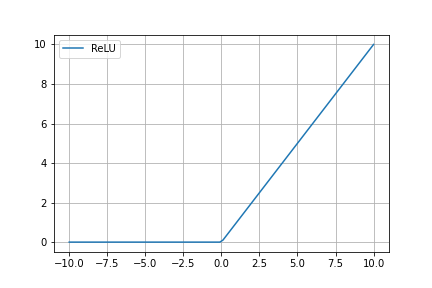
\includegraphics[scale=0.6]{img/relu.png}
  \caption{Grafico della ReLU.}
  \label{fig:relu}
\end{figure}


\begin{figure}[h!]
  \hspace*{0.9in}
  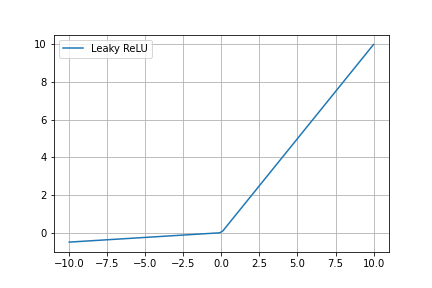
\includegraphics[scale=0.6]{img/leaky_relu.png}
  \caption{Grafico della Leaky ReLU.}
  \label{fig:leaky_relu}
\end{figure}






\subsection{Softmax}
Nei problemi di classificazione multiclasse, dove il numero di classi è maggiore di due, nello strato di output della rete non può essere usata la funzione sigmoid, che invece viene usata in ambito di classificazione binaria. Similarmente alla sigmoid, l'output della softmax può essere interpretato come le probabilità associate ad ogni classe, infatti tutti i valori sommati restituiscono 1. Quando il numero di classi è uguale a due, la softmax è equivalente alla sigmoid e volendo si può considerare la sigmoid un particolare caso della softmax o, in modo equivalente, la softmax una generalizzazione della sigmoid.
Di seguito la formula della softmax.
\\

\begin{equation}
softmax(x_{i}) = \frac{e^{x_{i}}}{\sum_{j}{e^{x_{j}}}}.
\end{equation}





\section{Apprendimento}
La fase di apprendimento è una fase in comune a tutti gli algoritmi di ML. In generale, in questa fase il modello che viene addestrato aggiorna i propri parametri cercando di migliorare le proprie performance, ovvero cercando di approssimare nel miglior modo possibile il pattern d'interesse.

\subsection{Paradigmi di apprendimento}
Nel campo del ML, esistono quattro principali paradigmi di apprendimento:

\begin{itemize}
    \item \textit{Supervisionato}: come detto in precedenza, l'approccio del ML si differenzia dall'approccio tradizionale nel fatto che chi sviluppa il modello non definisce le regole di funzionamento del mondo d'interesse, ma piuttosto si occupa di costruire un'architettura in grado di apprenderle dai dati. Detto ciò, risulta critico il ruolo dei dati. Infatti, soprattutto nel campo del DL dove i pattern del mondo d'interesse sono molto complessi, è fondamentale fornire al modello dati di quantità sufficiente, oltre che rappresentativi. In questo paradigma viene fornito al modello un insieme di dati, chiamato \textit{dataset}, composto da sole coppie di tipo X e Y, dove la X rappresenta l'input e la Y rappresenta il corretto output. Le coppie che compongono il dataset vengono utilizzate dal modello come esempio del funzionamento del pattern che sta cercando di approssimare.
    
    \item \textit{Non supervisionato}: in questo paradigma invece, nel dataset fornito c'è solo l'input senza il corretto output. Chiaramente, questo paradigma viene utilizzato solamente quando ottenere le corrispondenti label non è possibile oppure molto difficile. Un esempio di ciò è il campo delle immagini mediche, in cui solo degli specialisti possono produrre le label. Un altro esempio è quando la loro produzione risulta un processo molto lungo e tedioso, cosa che avviene spesso nell'ambito della segmentazione. Quando questo succede e il modello non ha esempi di input-output su cui basarsi, l'approccio più tipico è quello di cercare negli elementi del dataset delle similarità, in modo da poterli raggruppare in quelli che vengono chiamati \textit{cluster}.
    
    \item \textit{Semi Supervisionato}: questo paradigma è un punto d'incontro tra il paradigma supervisionato e quello non supervisionato. In particolare, in questo caso solo ad una parte del dataset è associata la corrispondente label.
    
    \item \textit{Per rinforzo}: qui il modello, detto anche \textit{agente}, apprende interagendo con l'ambiente esterno. In particolare, l'agente compie delle azioni e successivamente ne valuta i risultati, utilizzando un valore numerico di "ricompensa", che ha l'obiettivo di incoraggiare azioni correte e scoraggiare quelle scorrette.

\end{itemize}

\subsection{Funzioni di perdita}
Nella fase di apprendimento, un aspetto critico è come il modello valuta le proprie performance. In particolare, ad ogni iterazione dell'apprendimento il modello deve avere la capacità di valutare quanto il suo output sia distante da quello corretto. Di conseguenza, il modello per apprendere ha bisogno di una misura di questa distanza. Questo ruolo è ricoperto dalla funzione di perdita, che viene decisa dagli sviluppatori prima della fase di addestramento. La scelta della funzione di perdita è fondamentale e può avere un grande impatto sulle performance del modello. Una caratteristica fondamentale della funzione di perdita è la derivabilità. In particolare, è fondamentale in quanto la sua derivata viene utilizzata proprio per addestrare la rete (entremo nel dettaglio sul meccanismo di apprendimento più avanti). Di funzioni di perdita ne esistono molte tipologie che vengono scelte in base, soprattutto, al task:
\begin{itemize}
    \item nei problemi di regressione, ovvero dove l'output è un valore all'interno di un intervallo continuo, una delle funzioni di perdita più comuni è la \textit{MSE (Mean Squared Error)}, che calcola la media delle differenze al quadrato tra gli elementi del vettore delle predizioni \textit{pred} e gli elementi del vettore di output corretto \textit{y}.
    
    \begin{equation}
    MSE = \frac{1}{n}\sum_{y=1}^{n}(pred_{i} - y_{i})^{2}.
    \end{equation}

    \item nei problemi di classificazione binaria, una delle più utilizzate è la \textit{Binary Cross Entropy}.
    
    \begin{equation}
    BCE = -\frac{1}{n}\sum_{i=1}^{n}{(y_{i}\log(pred_{i}) + (1 - y_{i})\log(1 - pred_{i}))}.
    \end{equation}
    
    \item nei problemi di classificazione multiclasse, invece, viene spesso utilizzata la Cross Entropy
    \begin{equation}
    CE = -\frac{1}{n}\sum_{i=1}^{n}y_{i}\log(pred_{i}).
    \end{equation}
    
\end{itemize}

%\subsubsection{Focal Loss}
%Uno dei problemi che spesso emerge nell'affrontare un task di classificazione, rispetto a uno di regressione, è il bilanciamento delle classi del dataset. In particolare, questo problema sorge quando il numero di elementi del dataset appartenenti a una classe sono molti di più rispetto a quelli appartenenti ad un altra classe. Nel caso della segmentazione semantica, questo si trasforma nel avere classi a cui appartengono grandi porzioni delle immagini e classi a cui invece appartengono pochi pixel. Per esempio, nel dataset usato in questo lavoro, la classe \textit{prato} è molto presente e spesso ricopre una gran parte delle immagini, mentre la classe \textit{veicolo} è molto poco presente, sia a livello di numero di immagini in cui sono presenti veicoli sia a livello di numero di pixel che una veicolo ricopre. Il problema, è che le reti neurali che vengono addestrate su dataset che presentano questa caratteristica, spesso poi sono performanti nel riconoscere la classe più presente ma ottengono scarsi risultati nel riconoscere quella meno presente.
%Questo problema si può risolvere in diversi modi. Uno delle soluzioni più utilizzate è la funzione di perdita pesata, ovvero applicare ad ogni classe un peso che rappresenti l'importanza di riconoscere quella determinata classe. In particolare, alle classi più presenti vengono attribuiti pesi più bassi e a quelle meno presenti pesi più alti, in modo che, durante l'addestramento vengano più enfatizzati gli errori commesssi nel riconoscere classi meno presenti. Un esempio di questa tecnica utilizzata è la Cross Entropy Pesata, variante della funzione sopra menzionata.

%Durante questo lavoro, il problema dello sbilancimento delle classi del dataset, è stato uno dei principali problemi da affrontare e per risolverlo è stata utilizzata un particolare funzione di perdita chiamata \textit{Focal loss} \cite{focalloss}.








\subsection{Retropropagazione dell'errore}
Nelle reti neurali, così come in quasi tutti gli algoritmi di ML, la fase di apprendimento è una fase iterativa. Ad ogni iterazione, la rete, con i suoi parametri attuali, elabora uno o più elementi del dataset, confrontando poi l'output con la label corretta attraverso la funzione di perdita. A questo punto, la rete aggiorna i propri i parametri cercando di migliorare. Per capire come dovrebbe essere lo strato di output, abbiamo dei valori di riferimento, mentre per gli strati nascosti non abbiamo una diretta indicazione. L'aggiornamento dei parametri, generalizzata sia per lo strato di output che per quelli nascosti, è descritta dalla \textit{regola delta}:

\begin{equation}
\Delta w_{jk} = -\eta \delta _{j}o_{k}.
\end{equation}

Dove $\Delta w_{jk}$  è la variazione dei parametri tra il neurone $k$ e $j$, $\eta$ è il learning rate, $o_{k}$ è l'output dl neurone $k$, ovvero l'input del neurone $j$ e $\delta _{j}$ è l'errore dell'output del neurone $j$. La differenza tra strato d'output e strato nascosto sta nel valore di $\delta _{j}$, ovvero per lo strato d'output è il seguente

\begin{equation}
\delta _{j} = y_{j}(1-y_{j})(o_{j} - y_{j}).
\end{equation}

Dove $o_{j}$ è l'output del neurone $j$, mentre $y_{j}$ è l'output corretto.
Dall'altra parte, per gli strati nascosti è equivalente a 

\begin{equation}
\delta _{j} = y_{j}(1-y_{j})\sum_{k}\delta _{k}w_{kj}.    
\end{equation}

Dove invece $\sum_{k}\delta _{k}w_{jk}$ è la somma pesata degli errori di tutti i neuroni collegati a $j$. Infine, tutti i neuroni aggiornano i propri parametri utilizzando la seguente formula:

\begin{equation}
w_{jk} = w_{jk} + \Delta w_{kj}.
\end{equation}







\section{Regolarizzazione}
\label{regolarizzazione}
In generale, nel campo del Machine Learning, così come nel campo dell'ottimizzazione di funzioni, quello che si cerca di fare è minimizzare una funzione, o in altri termini, minimizzare un errore. La principale differenza tra i due campi è che, nel ML, oltre all'errore sul training set (\textit{training error}), viene anche preso in considerazione il \textit{test error}, anche detto "errore di generalizzazione". In particolare, alla fine della fase di addestramento, è importante che il modello costruito abbia delle buone performance non solo sui dati di addestramento (training set), ma anche e soprattutto su dati mai visti (test set) e questa abilità viene chiamata generalizzazione.
La capacità di un modello di saper generalizzare è molto importante e può dipendere da molti fattori. In particolare, oltre che dal giusto metodo e quantità di addestramento, dai giusti iperparametri e da molti altri fattori, la generalizzazione può soprattutto dipendere dalla scelta della complessità del modello. In generale, per quanto riguarda la complessità, il modello si può trovare in tre situazioni: nella prima il modello non ha approssimato bene il pattern interessato e la sua complessità è troppo bassa (\textit{underfitting}), nella seconda invece il modello è riuscito a cogliere il vero pattern e infine, nella terza situazione, il modello costruito ha alzato troppo la sua complessità, approssimando un pattern più complesso ma che include quello interessato (overfitting) (Figura \ref{fig:under-overfitting}). 

\begin{figure}[h!]
  \hspace*{-0.2in}
  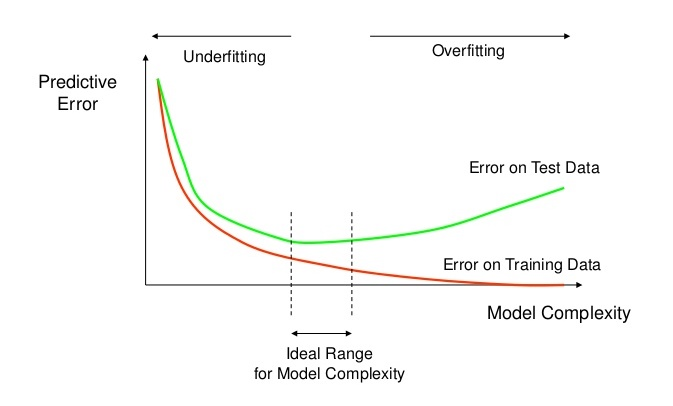
\includegraphics[scale=0.6]{img/over_underfitting.jpeg}
  \caption{Grafico degli errori sul training set e sul test set in funzione della complessità del modello e illustrazione dei due stati di underfitting e overfitting.}
  \label{fig:under-overfitting}
\end{figure}


Nel caso della prima situazione ci sono diverse soluzioni, ma in generale vanno riviste le scelte di design del modello e in ogni caso va aumentata la sua complessità. Nel caso dell'overfitting, invece, un metodo molto utilizzato è quello della regolarizzazione, il cui obiettivo è proprio quello di portare il modello dalla terza alla seconda situazione. In generale, possiamo definire la regolarizzazione come qualsiasi modifica che apportiamo al nostro modello o all'algoritmo di apprendimento, con l'obiettivo di ridurre il suo errore di generalizzazione ma non quello di addestramento.
Spesso nella pratica, soprattutto nei campi di applicazione del Deep Learning, anche con un un modello molto complesso, non è detto che si riesca ad includere il pattern interessato. In particolare nel mondo del DL, i modelli sono applicati a domini estremamente complessi e, di conseguenza, quasi sicuramente il vero pattern è al di fuori di quello del modello. Questo comporta che nella maggior parte dei casi, la scelta migliore è quella di grandi modelli con un'alta complessità, affiancati dalle giuste tecniche di regolarizzazione \cite{goodfellow2016deep}.
\\ \\
Di tecniche di regolarizzazione ne esistono svariate, ma uno dei metodi generali più utilizzati è quello di limitare la complessità del modello, anche detta capacità, aggiungendo alla funzione di perdita una componente di penalità $\Omega(W)$, trasformando la funzione di perdita, o anche detta funzione obiettivo, $J(W; X,y)$ in $\tilde{J}(W; X,y)$ dove:

\begin{equation}
    \tilde{J}(W; X,y) = J(W; X,y) + \alpha\Omega(W).
\end{equation}

Dove $\alpha\in[0, \infty] $ è un iperparametro che rappresenta il peso del contributo della penalità, $W$ sono i parametri del modello, $X$ rappresenta i dati di training e $y$ l'output corretto. In particolare, questa componente rappresenta l'intenzione di voler penalizzare la complessità del modello, di conseguenza, con la sua aggiunta durante la fase di apprendimento, l'algoritmo non cerca solo di minimizzare il training error, ma anche la complessità del modello. Nel dettaglio, esistono diversi metodi di questo genere e in ognuno $\Omega(W)$ prende una diversa forma. Due dei metodi più noti ed utilizzati di questa categoria sono la regolarizzazione L1 e la regolarizzazione L2. Un altro metodo di regolarizzazione molto usato nelle reti neurali è il \textit{dropout}. Il funzionamento di questa tecnica è molto semplice e intuitivo: durante l'addestramento, con una certa probabilità $p$, alcuni nodi della rete vengono disattivati, trasformando così a tutti gli effetti la rete in una meno complessa e riducendo la sua complessità (Figura \ref{fig:dropout}). Nel dettaglio, così come anche le altre tecniche di regolarizzazione menzionate prima, il dropout tende a tenere i parametri del modello  più bassi possibili e lo fa evitando di far prevalere un nodo sugli altri. In particolare, disattivando a turno randomicamente i vari nodi, costringe la rete a non sbilanciare i propri parametri verso un nodo, ottenendo dei parametri più bilanciati e di conseguenza più piccoli, mentre senza il dropout, il rischio è che durante l'addestramento la rete possa aumentare di molto i parametri di un nodo e azzerare quelli di altri.

\begin{figure}[h!]
  \hspace*{0.4in}
  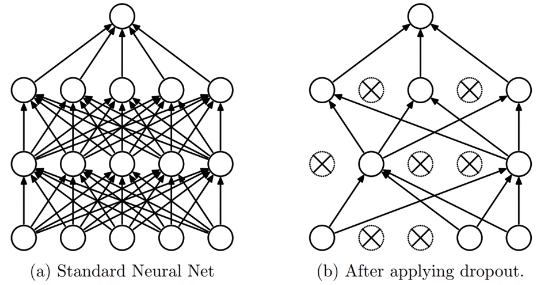
\includegraphics[scale=0.6]{img/dropout.png}
  \caption{Illustrazione della tecnica di dropout.}
  \label{fig:dropout}
\end{figure}




\subsection{Data augmentation}
\label{data_augmentation}
A parte le tecniche di regolarizzazione, il metodo sicuramente migliore per aumentare la capacità di generalizzazione di un modello è quello di fornigli più dati in input. Purtroppo però, come già detto, nella pratica i dati sono spesso molto difficili da reperire, soprattutto in alcuni campi di applicazione del DL. Spesso, per sopperire a questa difficoltà, si fa uso di una famiglia di tecniche di regolarizzazione chiamata \textit{data augmentation}. In generale, per data augmentation si intende una qualsiasi tecnica con cui si producono dati finti, partendo  da quelli veri. In particolare, partendo da uno o più elementi del dataset e applicando una trasformazione di qualche tipo, si può produrre un dato artificiale, ma comunque realistico. Questa tecnica viene spesso utilizzata nel campo della Computer Vision, dove le trasformazioni applicate ai dati sono ad esempio rotazioni, traslazioni, modifica del contrasto o della luminosità e molti altri (Figura \ref{fig:example-data_aug}). In questo campo, per alcuni task come la classificazione, la tecnica del data augmentation risulta spesso molto semplice, in quanto, dato che i classificatori devono risultare invarianti rispetto a molte trasformazioni dei dati \cite{goodfellow2016deep}, le trasformazioni fatte durante la data augmentation vanno applicate solamente alle immagini e non alle label, che invece devono rimanere uguali, cosa non vera, invece, nel campo della segmentazione semantica, dove andrebbero applicate in modo equo anche alle maschere.

\begin{figure}[h!]
  \hspace*{0.1in}
  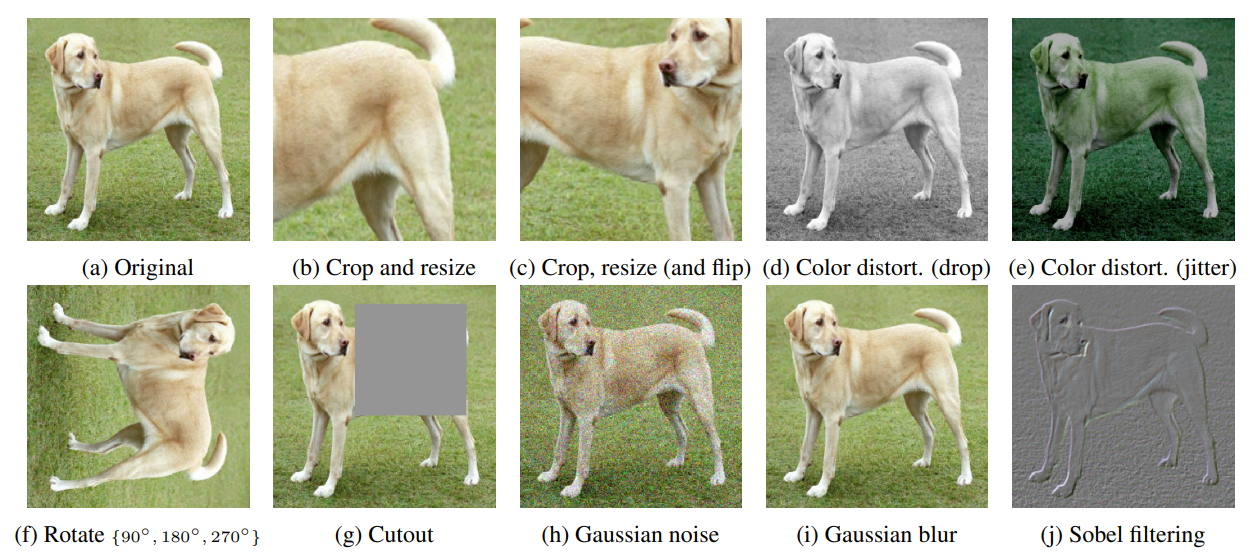
\includegraphics[scale=0.3]{img/example_data_aug.png}
  \caption{Alcuni esempi delle possibili trasformazioni per applicare data augmentation a un dataset d'immagini.}
  \label{fig:example-data_aug}
\end{figure}

Un'altra tipologia di data augmentation molto utilizzata è la \textit{noise injection}, ovvero la tecnica nella quale viene randomicamente applicato un certo rumore ai dati del dataset. Questa tecnica risulta spesso molto importante, poiché l'invarianza dei modelli rispetto al rumore nel dato in input è una caratteristica molto importante e desiderata, e la sua mancanza può portare a dei risultati negativi \cite{deep_trouble}, anche nell'ottica dell'Explainable AI. In particolare, spesso le immagini con l'aggiunta di un certo tipo di rumore risultano agli occhi umani identiche a quelle originali, di conseguenza il variare dell'output del modello da un'immagine all'altra può risultare un problema per l'interpretabilità del modello.
\\
Come precedentemente menzionato, la data augmentation risulta più semplice  per alcuni task, mentre per altri meno. Inoltre, recenti ricerche \cite{data_aug_effects} hanno dimostrato che questa tecnica può, da un lato portare a grandi miglioramenti nella capacità del modello di generalizzare, dall'altro penalizzare alcune classi. In particolare, i suoi effetti sono \textit{class-dependent}, ovvero dipendono dalla natura delle classi del dataset, di conseguenza l'utilizzo di queste tecniche può portare a miglioramenti in alcune classi, ma anche ad un calo delle performance in altre, soprattutto quando si applicano le stesse trasformazioni all'intero dataset.









\section{Reti Neurali convoluzionali}
Le reti convoluzionali \cite{convnets}, come il percettrone multistrato, presentano un layer d'input, uno di output e diversi layer nascosti. La differenza tra le reti classiche e quelle convoluzionali sta proprio nella presenza, tra quelli nascosti, degli strati convoluzionali (Figura \ref{fig:conv_net}). In particolare, le convoluzioni sono delle matrici la cui dimensione viene decisa in anticipo, che rappresentano dei filtri che vengono applicati sull'immagine scorrendo su di essa per estrarre determinati pattern. Uno dei principali vantaggi è che scorrendo sull'immagine, la convoluzione è in grado di riconoscere il pattern che ha appreso durante l'addestramento indipendentemente dalla posizione nell'immagine, a differenza delle normali reti neurali dove i neuroni, in particolare i primi, sono associati a precise porzioni dell'immagine. 

\begin{figure}[h!]
  \hspace*{0.1in}
  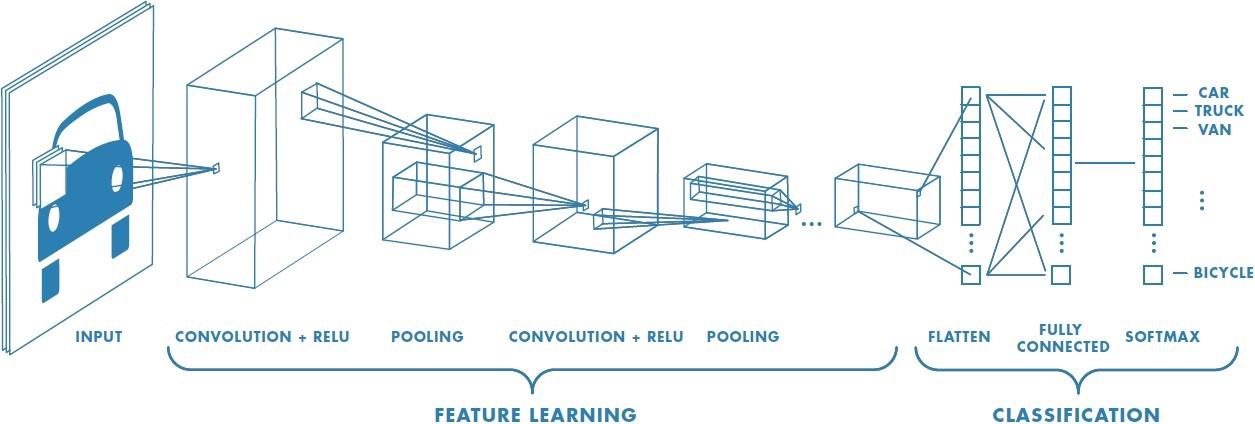
\includegraphics[scale=0.3]{img/conv_net.jpeg}
  \caption{Architettura di una generica rete convoluzionale.}
  \label{fig:conv_net}
\end{figure}

Le convoluzioni applicate alle immagini, anche chiamate \textit{kernel}, arrivano dal mondo della Computer Vision, dove vengono utilizzate per il processamento delle immagini. La differenza tra le convoluzioni tradizionali e quelle usate nelle reti neurali, sta nel fatto che mentre i valori di quelle tradizionali sono scelti in anticipo e pensati per applicare un determinato filtro, quelle nelle reti partono con dei valori inizializzati randomicamente, ed è proprio con l'addestramento che la rete impara quali sono i pattern da evidenziare. All'interno di una rete convoluzionale, solitamente, ci sono più strati convoluzionali e andando avanti nella rete, l'immagine in input diminuisce nelle prime due dimensioni (altezza e larghezza) e aumenta nella terza dimensione, ovvero quella del numero di feature, spesso chiamate canali. In particolare, ogni convoluzione applicata ad un'immagine produce una feature e più si va verso lo strato d'output, più le feature rappresentano pattern di più alto livello. Infatti, nei primi strati le feature rappresentano pattern più elementari, ad esempio forme geometriche come punti o linee. Negli strati più profondi invece, rappresentano strutture geometriche più complesse, oppure strutture con un significato semantico. La Figura \ref{fig:features} illustra in modo intuitivo il concetto appena spiegato.

\begin{figure}[h!]
  \hspace*{0.3in}
  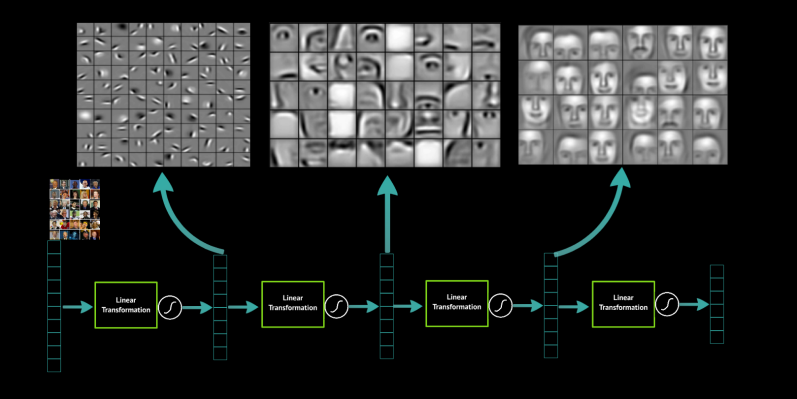
\includegraphics[scale=0.45]{img/features.png}
  \caption{Illustrazione del concetto di features di basso e alto livello.}
  \label{fig:features}
\end{figure}


Nella fase di costruzione della rete o successivamente nella fase di ottimizzazione degli iperparametri, riguardo le convoluzioni vanno stabiliti i valori di tre iperparametri:
\begin{itemize}
    \item \textit{dimensione del kernel}: la dimensione della matrice della convoluzione.
    
    \item \textit{stride}: indica il numero di pixel con cui la finestra si muove ad ogni operazione.
    
    \item \textit{padding}: denota il processo di aggiunta di zeri a ciasciun lato dell'input e questo iperparametro indica quanti aggiungerne. In particolare, il padding ha lo scopo di poter passare il kernel anche sui pixel più vicini ai bordi, e gli zero aggiunti servono proprio a riempire la parte del kernel che esce dall'input (Figura \ref{fig:padding}).
\end{itemize}

\begin{figure}[h!]
  \hspace*{1.7in}
  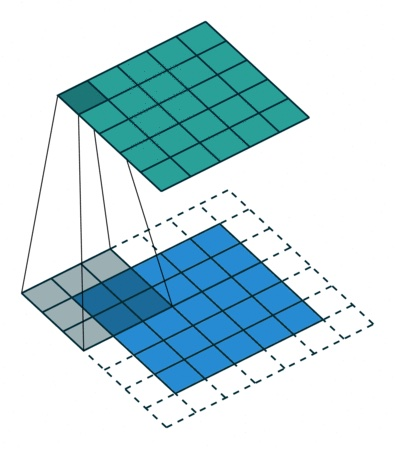
\includegraphics[scale=0.4]{img/padding2.jpg}
  \caption{Illustrazione del padding.}
  \label{fig:padding}
\end{figure}

Oltre agli strati convoluzionali, solitamente ci sono altre quattro tipologie di strati in una rete convoluzionale:
\begin{itemize}
    \item \textit{strato di pooling}: questo strato ha il ruolo di ridurre le prime due dimensioni del dato che attraversa la rete e anch'esso è un sorta di finestra che scorre sull'immagine, dando in output uno scalare. Ne esistono diverse tipologie, ma in generale, per una finestra dell'input restituisce un valore statistico di quest'ultima. Una delle tipologie più utilizzate è il \textit{max pool}, che restituisce il valore massimo all'interno della finestra; un altro molto usato è l'\textit{average pool}, che invece restituisce la media di tutti i valori nella finestra. A differenza della convoluzione, lo strato di pool non ha parametri apprendibili e il suo unico parametro è la dimensione della finestra, che più aumenta più riduce l'altezza e la larghezza del dato. L'importanza dello strato di pooling sta nel fatto che fornisce allo strato successivo l'invarianza rispetto a piccole traslazioni dell'input, ovvero modificando leggermente l'input dello strato di pooling, la maggior parte del suo output rimane invariato. Questa invarianza è fondamentale, soprattutto in alcuni task come la classificazione, in cui non è tanto importante dove sia la feature, ma piuttosto la sua presenza.
    
    \item \textit{strato di attivazione}: questa è una tipologia di strato in comune con tutte i tipi di rete neurale. Infatti, come già detto, questo strato ha il ruolo di fornire la non linearità alla rete, fondamentale per approssimare pattern complessi. Nel caso delle reti convoluzionali, la funzione di attivazione più comune è la ReLU e segue spesso gli strati di convoluzione.
    
    \item \textit{strato completamente connesso}: questa tipologia di strato, anche chiamato strato denso, è a tutti gli effetti strutturato come un percettrone multistrato e si trova sempre alla fine della rete. Questa parte della rete è la parte responsabile della classificazione, ovvero le feature ad alto livello prodotte dai primi strati vengono passate in input ai neuroni dello strato completamente connesso, così da produrre l'output finale.
    
    \item \textit{strato di attivazione finale}: questo strato rappresenta l'ultimo strato della rete ed ha il ruolo di traslare l'output nel range desiderato. Le due tipologie più utilzzate sono la \textit{sigmoid}, nel caso di classificazione binaria, e la softmax, nel caso di classificazione multiclasse.
\end{itemize}



\subsection{Reti neurali convoluzionali avanzate}

\subsubsection{VGG}
Il lavoro \cite{vgg}, che propose nel 2014 l'architettura chiamata VGG (Visual Geometry Group, ovvero il nome del gruppo di ricerca del lavoro) investigò il ruolo della profondità delle architetture nelle performance delle reti convoluzionali. Da questo studio ne risultò una delle architetture più note nel campo delle reti convoluzionali e della Computer Vision. Per quanto riguarda la struttura generale dell'architettura (Figura \ref{fig:vgg}), che però presenta diverse versioni a seconda della profondità, è composta da un primo strato, ovvero quello che prende in input l'immagine, che ha una dimensione fissa di 224x224, di conseguenza con questa versione della rete, tutte le immagini date in input devono avere quella dimensione e questo aspetto è dovuto al fatto che alla fine della rete sono presenti degli strati densi, anche detti \textit{fully connected} (FC), che non permettono alla rete di avere input di dimensioni diverse. Dopodichè, questo primo strato è seguito da uno stack di strati di convoluzioni 3x3, insieme, chiaramente, agli strati della funzione di attivazione (ReLU), con stride 1 e padding 1 (in modo da preservare la risoluzione spaziale dopo la convoluzione). In alcuni strati della rete sono presenti gli strati di pooling (max pooling), in particolare, in totale sono 5 e presentano una finestra 2x2 con stride 2. Infine, l'ultima parte della rete è composta da tre strati densi, di cui il primo e il secondo hanno una dimensione di 4096 canali, mentre l'ultimo ne ha 1000, poichè è stata costruita per essere testata su ImageNet che ha 1000 classi e un ultimo strato di Softmax.


\begin{figure}[h!]
  \hspace*{0.4in}
  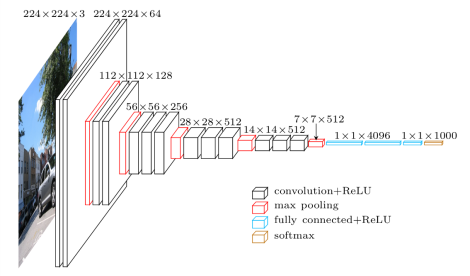
\includegraphics[scale=0.7]{img/vgg.png}
  \caption{Architettura generica della VGG.}
  \label{fig:vgg}
\end{figure}


Come detto precedentemente, l'architettura appena descritta assume diverse forme a seconda della profondità dello stack di convoluzioni. In particolare, le diverse versioni vanno da un minimo di 11 strati (8 strati di convoluzioni e 3 strati densi) fino ad un massimo di 19 (16 strati di convoluzioni e 3 strati densi), mentre l'ampiezza della rete (numero di canali) rimane coerente in tutte le versioni: parte da 64 fino ad arrivare negli ultimi strati di convoluzioni a 512.
La differenza principale tra la VGG e le architetture precedenti è soprattutto l'uso di convoluzioni piccole. In particolare, precedentemente la tendenza era quella di aumentare il campo ricettivo con convoluzioni sempre più grandi, come ad esempio nell'AlexNet \cite{alexnet}, che usa convoluzioni 11x11 con stride 4, oppure nell'archittetura proposta in \cite{visualizing_cnns} e nella OverFeat di \cite{overfeat}, che usano convoluzioni 7x7 con stride 2.
I vantaggi che gli autori di \cite{vgg} evidenziano riguardo l'uso di convoluzioni 3x3, sono principalmente dovuti al fatto che lo stesso campo ricettivo prodotto da una convoluzione 7x7 è riproducibile con uno stack di tre convoluzioni 3x3, con il vantaggio di incorporare tre strati di attivazione, che rende la funzione totale più discriminativa, e al fatto che in questo modo si riducono il numero di parametri della rete. In particolare, uno stack di tre convoluzioni ha $3(3^{2}C^{2})=27C^{2}$ parametri, dove $C$ è il numero di canali dell'input, mentre una convoluzione 7x7 ha $7^{2}C^{2}$ parametri.






\subsubsection{DenseNet}
Un'altra delle architetture più note è la DenseNet \cite{densenet}, un modello di rete convoluzionale ispirato al modello \textit{feed-forward}. In particolare, la peculiarità della DenseNet è che, a differenza delle classiche reti convoluzionali all'interno delle quali con $L$ strati si hanno $L$ collegamenti, ovvero uno tra ogni strato e il suo successivo, questa architettura  presenta $\frac{L(L+1)}{2}$ collegamenti, ovvero uno tra ogni strato e tutti gli strati successivi (Figura \ref{fig:densenet}).

\begin{figure}[h!]
  \hspace*{0.6in}
  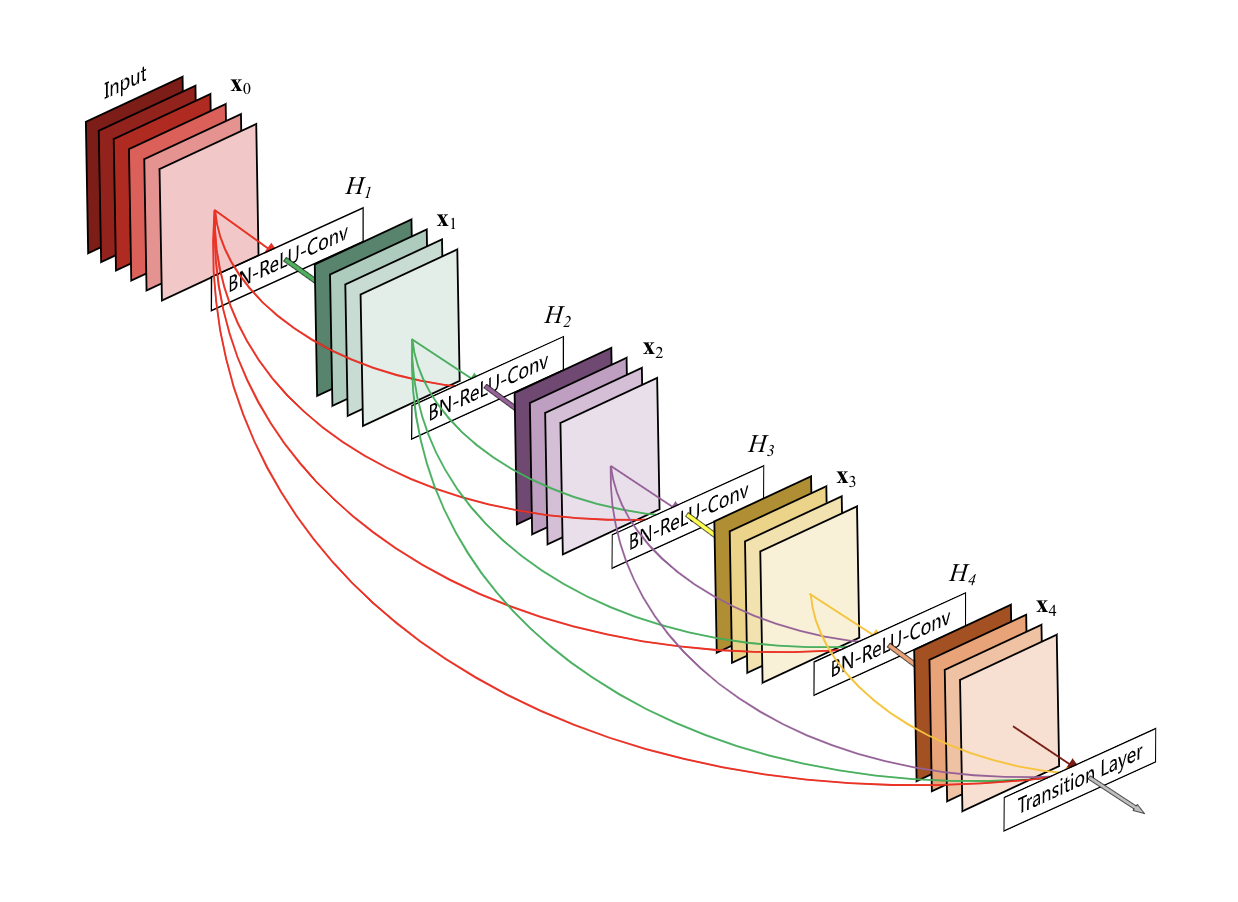
\includegraphics[scale=0.5]{img/densenet.png}
  \caption{Struttura di un blocco della DenseNet: ogni strato prende in input gli output di tutti gli strati precedenti \cite{densenet}.}
  \label{fig:densenet}
\end{figure}


I vantaggi evidenziati dagli autori di \cite{densenet} sono soprattutto riguardo uno dei maggiori problemi presenti nel campo delle reti neurali, ovvero la scomparsa del gradiente (\textit{vanishing gradients} in inglese). Come già menzionato, questo problema riguarda il fatto che nel meccanismo di retropropagazione dell'errore, quando si ha una rete molto profonda, si rischia che l'informazione sul gradiente, che viaggia dagli ultimi strati della rete fino ai primi, svanisca passando attraverso gli strati e non arrivi ai primi. In realtà, lo stesso problema può essere visto da un'altra prospettiva, ovvero nelle reti molto profonde non sono solo le informazioni sul gradiente a rischiare di scomparire, ma anche le informazioni sull'input che viaggiano dai primi agli ultimi strati. Nel corso degli anni, fino alla pubblicazione della DenseNet, in altri lavori \cite{resnets, huang2016deep, srivastava2015training, larsson2016fractalnet} questo problema è stato affrontato con diverse tecniche, che però hanno tutte avuto una cosa in comune, ovvero l'utilizzo di brevi connessioni per connettere strati vicini. Il lavoro fatto dagli autori, infatti, ha cercato di distillare e generalizzare questi approcci proposti precedentemente, creando un semplice schema di connessioni con l'obiettivo di massimizzare il flusso di informazioni tra gli strati della rete. Inoltre, a differenza di \cite{resnets}, la DenseNet, per minimizzare la perdita delle informazioni che giungono da strati precedenti, non utilizza la somma come operazione di fusione di diversi input, bensì la concatenazione.







\subsubsection{Modulo Inception e GoogLeNet}
Il lavoro \cite{inception}, seguendo la tendenza di quegli anni di aumentare sempre di più la complessità delle reti convoluzionali per aumentare le perfomance, ha avuto l'obiettivo di trovare un metodo per aumentare la complessità delle reti, senza però aumentare il suo costo computazionale. In particolare, l'idea dietro il loro lavoro è stata quella di creare un modulo, chiamato modulo "Inception", all'interno del quale venissero utilizzate contemporaneamente tutte le tipologie di componenti (convoluzioni con diverse dimensioni, pooling, ...), che solitamente venivano alternate strato per strato. L'intuizione di questo meccanismo è che la scelta dell'operazione da utilizzare per ogni strato non è più di chi costruisce il modello, ma del modello stesso, che ad ogni strato non è più limitato all'informazione della singola operazione fatta in quello strato, ma ha a disposizione le informazioni risultato di diverse operazioni fatte sullo stesso input. In particolare, la scelta degli autori su quali operazioni fare in parallelo nel modulo Inception è ricaduta su: convoluzione 1x1, convoluzione 3x3, convoluzione 5x5 e infine max pooling. Questa scelta è frutto di esperimenti fatti su diverse combinazioni, che come risultato hanno giudicato questa come la migliore. In realtà però, nei successivi sono state  proposte diverse varianti e nuove versioni del modulo Inception, che hanno utilizzato diverse combinazioni \cite{inceptionv2, inceptionv3, inceptionv4, xception}. Entrando nel dettaglio del suo funzionamento, il modulo Inception si basa sul dare lo stesso input parallelamente alle quattro diverse operazioni, i cui risultati vengono poi concatenati e passati al prossimo strato (Figura \ref{fig:inception_module_naive}). Per concatenare i quattro diversi output, chiaramente le loro prime due dimensioni (altezza e larghezza) devono coincidere, per far questo le tre operazioni di convoluzioni hanno dei parametri di stride e padding mirati. Per quanto riguarda il maxpooling, invece, che a differenza della convoluzione riduce per forza altezza e larghezza dell'input, è necessaria una certa quantità di padding per rendere il suo output coerente con gli altri.

\begin{figure}[h!]
  \hspace*{0.5in}
  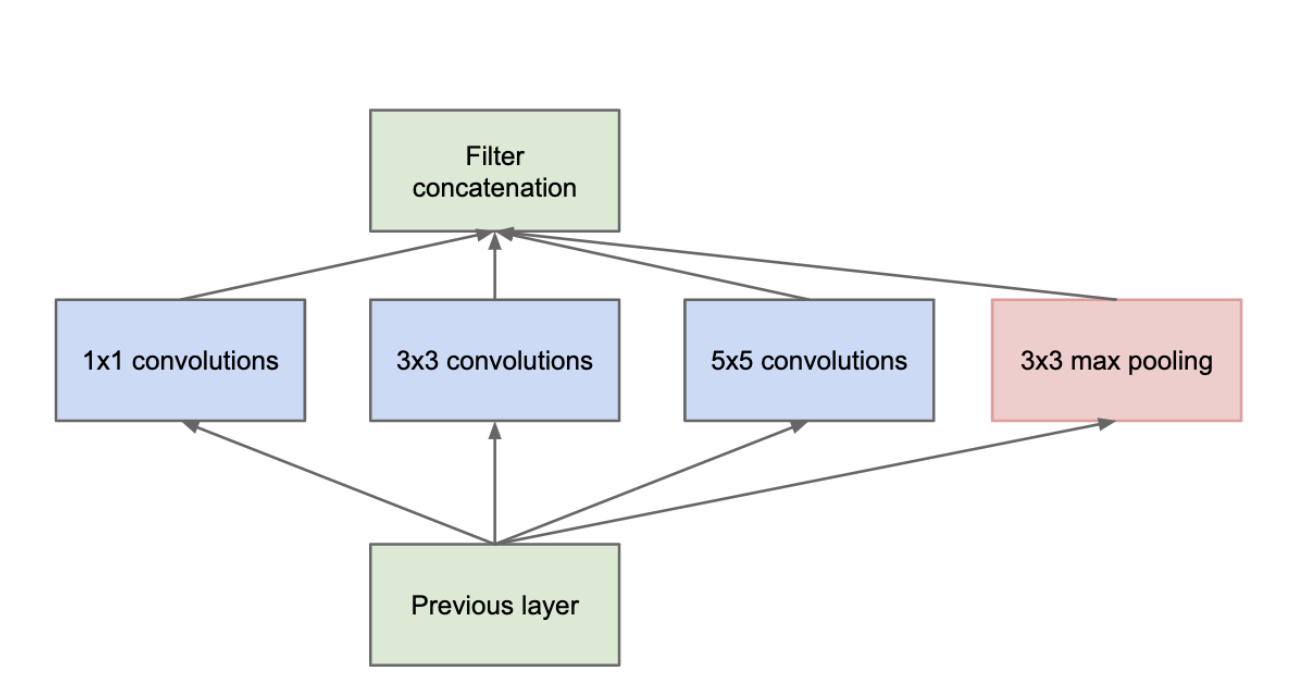
\includegraphics[scale=0.49]{img/inception-module_naive.png}
  \caption{Illustrazione del modulo Inception \cite{inception}, la versione senza riduzione delle dimensioni con costo computazionale molto alto.}
  \label{fig:inception_module_naive}
\end{figure}

Il problema di questa versione del modulo è che, aumentando di molto l'ampiezza degli strati della rete senza nessun tipo di accorgimento particolare,  anche il suo costo computazionale è aumentato. Per far fronte a questo aumento, gli autori hanno proposto un approccio che si basa sull'utilizzo di convoluzioni 1x1 per ridurre le dimensioni dell'input. In particolare, per le operazioni computazionalemente più costose, ovvero la convoluzione 3x3 e la convoluzione 5x5, aggiungono prima  una convoluzione 1x1, chiamata in questo caso \textit{bottleneck}, che ha lo scopo di portare l'input ad una dimensione per cui  applicare le convoluzioni ha un costo computazionale meno elevato. Inoltre, per quanto riguarda il maxpooling, la convoluzione 1x1 viene aggiunta dopo, dato che in questo caso non è tanto il costo computazionale dell'operazione a creare problemi, ma piuttosto la dimensione del suo output (che ha lo stesso numero di canali dell'input), il max pooling è seguito da una convoluzione 1x1, per far in modo di ridurre il numero di canali del suo output (Figura \ref{fig:inception_module}).

\begin{figure}[h!]
  \hspace*{0.6in}
  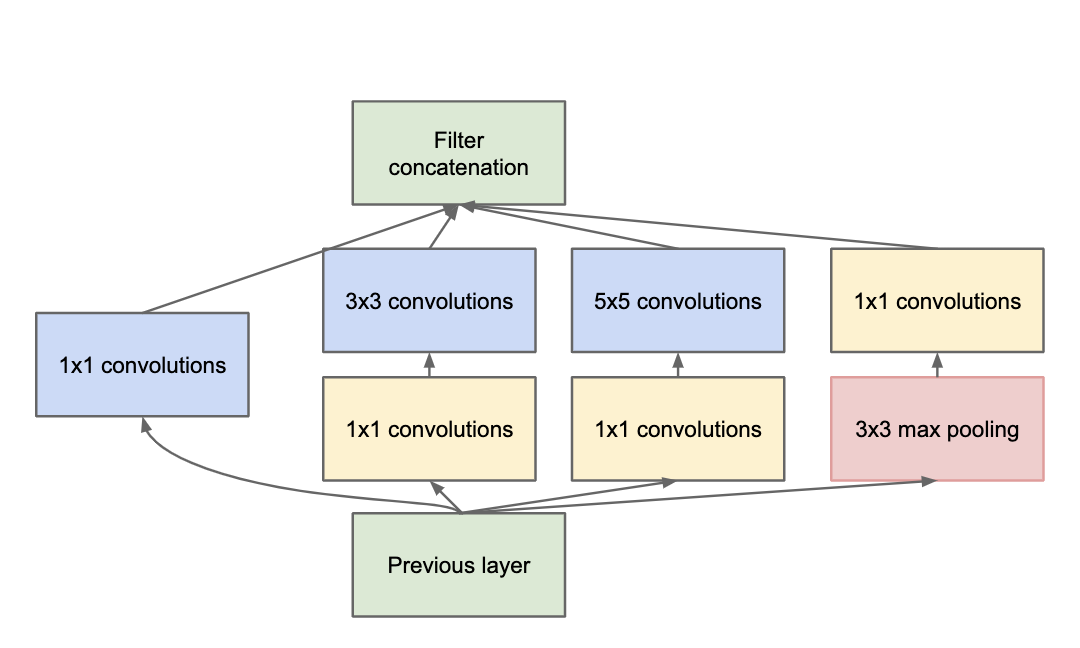
\includegraphics[scale=0.55]{img/inception.png}
  \caption{Illustrazione del modulo Inception \cite{inception}, la versione con la riduzione delle dimensioni attraverso strati di convoluzioni 1x1.}
  \label{fig:inception_module}
\end{figure}

Oltre alla concezione del modulo Inception, gli autori di \cite{inception} hanno anche proposto un'intera architettura basata proprio su questo tipo di modulo, la "GoogLeNet", il cui nome rende omaggio alla LeNet \cite{lenet}, una delle prime reti neurali convoluzionali sviluppate.
La GoogleNet (Figura \ref{fig:googlenet}), in particolare, è essenzialmente composta da uno stack di moduli Inception. Una sua peculiarità, al di là dell'uso del modulo Inception, è la presenza di due ulteriori strati intermedi di output. In particolare, la rete presenta in due dei moduli Inception dei rami addizionali di output, che terminano con uno strato di Softmax, trasformando l'output dei due strati intermedi in output effettivi della rete. A renderli due output effettivi della rete, è il fatto che la loss function totale, che la rete utilizza per addestrarsi, è calcolata con una somma pesata di tutti e tre gli output (questi due più quello finale), dando più peso a quello finale. Così facendo, la loss function  constringe la rete ad avere le feature map di quei due strati intermedi, già di una buona qualità per fare una predizione e l'idea dietro questo meccanismo è che si ottiene un effetto di regolarizzazione, spingendo la rete a non cadere nell'overfitting.


\begin{figure}[h!]
  \hspace*{1.3in}
  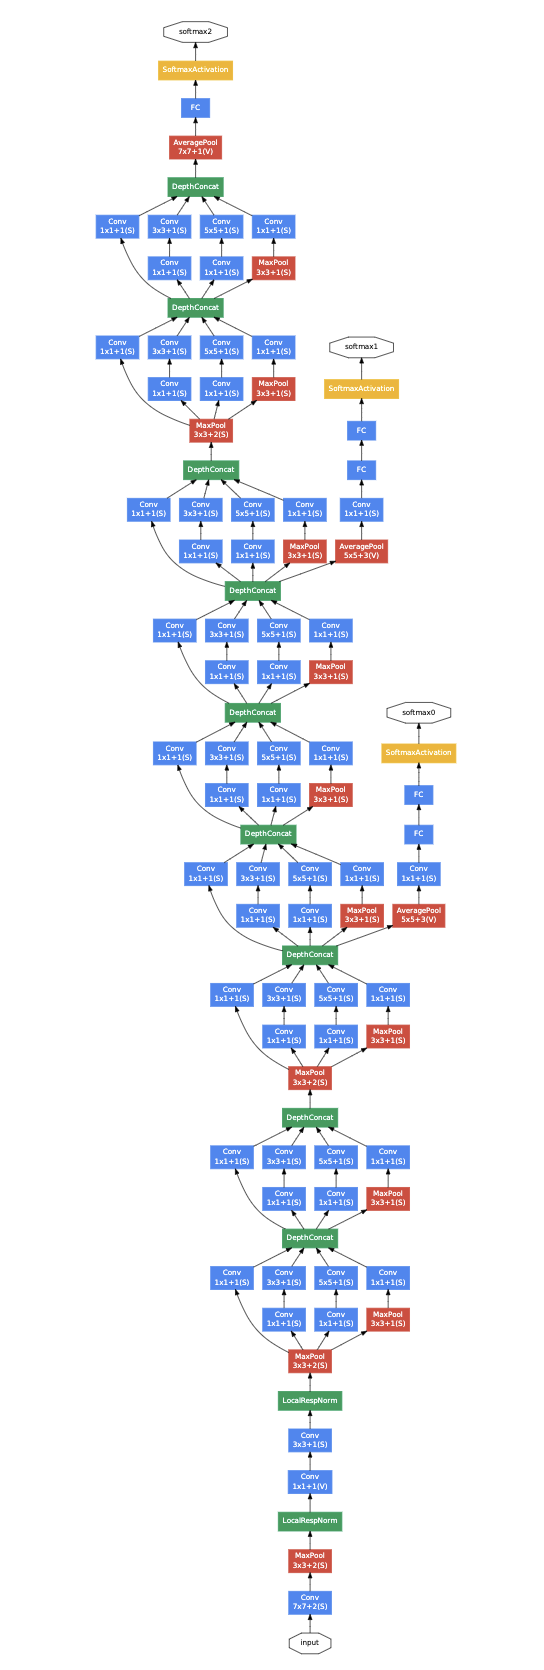
\includegraphics[scale=0.75]{img/googlenet.png}
  \caption{Architettura della GoogLeNet \cite{inception}.}
  \label{fig:googlenet}
\end{figure}



